\documentclass[a4paper, 12pt]{article}
\usepackage{cmap}
\usepackage[utf8]{inputenc}
\usepackage[english, russian]{babel}
\usepackage[left=2cm, right=2cm, top=2cm, bottom=2cm]{geometry}
\usepackage{amsfonts,amssymb}
\usepackage{amsmath}
\usepackage{amsthm}
\usepackage{titlesec}
\usepackage{graphicx}
\usepackage{mathtools}
\usepackage{hyperref}

 \newcommand{\tit}[1]{\begin{center}{\bf{\Large #1}}\end{center}}
 \newcommand{\aut}[1]{\centerline{{\bf #1}}}
 \newcommand{\cityorg}[1]{\centerline{\it #1}}
 \newcommand{\email}[1]{\centerline{{\small e-mail: #1}}\vspace{\baselineskip}}
\providecommand{\keywords}[1]{\textbf{\textit{Ключевые слова:}} #1}
\newcommand{\norm}[1]{\left\lVert#1\right\rVert}
\newcommand{\normb}[1]{\left\lVert\textbf{#1}\right\rVert}

\begin{document}

\sloppy
 \tit{Маскировка при помощи оптимизированных однородынх анизотропных слоев}
 \aut{Bogdan-Ioan Popa, Steven A. Cummer}

\begin{abstract}
Мы представляем метод уменьшения рассеяния произвольных объектов, заключающийся
в окружении их оболочкой, состоящей из нескольких слоев анизотропных однородных 
материалов. Для нахождения материальных параметров для каждого слоя используется
оптимизаионный метод, отправной точкой которого является дискретная аппроксимация
координатного преобразования маскирующей оболочки. Мы покажем, что оптимизированная
трехслойная оболочка может снизить рассеяние на целых 15дБ больше, чем 100 слойная
реализация маскирующей оболочки с преобразованием координат. Более того,
оптимизационный метод может решения высокопроизводительной маскировочной оболочки,
которые удовлетворяют внешним ограничениям, таким как максимальное значение
диэлектрической или магнитной проницаемости. Такой подход может значительно
упростить маскировочных оболочек среднего размера. 
\end{abstract}

Недавно значительные исследования сфокусировались на разработке новых
методов оптимизации взаимодействия между заданными объектами и электромагнитыми
волнами. Пендри и другие \cite{1} показали, что тщательно спроектированные
неоднородные и анизотропные оболочки могут препятствовать распостранению
электромагнитного излучения внутрь них, и, гораздо важнее, убирает рассеяние
этих оболочек, превращая их и их внутренность прозрачным для электромагнитных волн.
В преобразовании координат является привлекательным его общность: 
он может быть применен для сокрытия объектов любой формы и размера.

Несмотря на то, что численное моделирование \cite{2} и далее теоретический анализ
\cite{3} подтвердили эффективность этого метода, эксперементальные демонстрации
оказались более сложной задачей. Одна попытка \cite{4}, включающая цилиндрическую
оболочку, окружающую металлический цилиндр продемонстировала основную физику
таких структур, а именно, что волны можно напрвлять вокруг структуры. Однако,
в данной работе были сделаны приближения \cite{2}, значительно снижающие
эффективность оболочки. В другой работе были выведены различные аппроксимации
к идеальной маскировочной оболочке, которые также жертвуют производительностью
в пользу простоты изготовления \cite{5-7}.

Трудность построения маскировочных оболочек, заданных теорией преобразования
координат, вытекает из требований материала, их состовляющего: оболочка должна
быть анизотропной, с диэлектрической и магнитной проницаемостью непрерывно
изменяющимися в широком диапазоне значений. Физическая ее реализация 
всегда будет требовать некоторую форму дискретизации этих непрерывных профилей.
Например, Шуринг и другие \cite{4} в их эксперименте использовали десятислойную 
ступенчатую аппроксимацию идеальных параметров.

Начиная с идеи, что анизотропия, кажется, является самым важным ингридиентом
маскирующих оболочек, которые не являются электрически малыми, можно было бы
задаться вопросом, могут ли анизотпроные оболочки, состоящие из антизотропных 
слоев построены другим образом? Здесь мы покажем, что уменьшающие рассение
оболочки, составленные из относительного малого числа однородных слоев,
могут быть построены при помощи оптимизаионного метода, использующего 
оболочку, построенную по принципу преобразования координат в качестве начального 
условия.
Производительность менее чем 5 оптимизированных слоев может быть равной,
или даже превосходить стослойную дискретную аппроксимацию гладной однородной
оболочки, построенной через преобразование координат.

Для простоты, мы сосредоточим наше внимание на двумерной цилиндрической оболочке
для элекромагнетизма, но представленный здесь анализ может быть применем для
других геометрий и типов волн, таких, как акустические \cite{8}. На рис. 1
изображен идеальный электрический проводник --- цилиндрический объект радиуса
$a$, окруженный оболочкой с внешним радиусом $b$. Было показано \cite{2},
что один набор относительных материальных параметров, который может полностью
убрать рассеяние от структуры имеет вид (в цилиндрических координатах):

\begin{equation*}
	\epsilon_r(r) = \mu_r(r) = \frac{r-a}{r}, \qquad 
	\epsilon_\phi(r) = \mu_\phi(r) = \frac{r}{r-a},
\end{equation*}

\begin{equation}\label{e1}
	\epsilon_z(r) = \mu_z(r) = \left( \frac{b}{b-a}	\right)^2 \frac{r-a}{r},
\end{equation}

где $z$ --- инвариантное направление, а $r$ и $\phi$ --- ридиальная и азимутальная
координаты соответственно.

Мы рассматриваем только поперечно электрическую поляризацию, для которой
релевантны только $\epsilon_z, \mu_r$ и $\mu_\phi$. Предполоаем, что оболочка
может быть собрана из $M$ концентрических слоев однородного материала, как показано
на рис. 1. Каждый слой характеризуется тензорами диэлектрической и магнитной
проницаемости, являющимися постоянными внутри слоя. Наша цель заключается в 
нахождении набора параметров, который бы минимизировал рассеяние оболочки.
Один способ --- использовать поваговое приближение \eqref{e1}, как в \cite{4}.
Используя этот подход и TE поляризацию, как было указано нами ранее \cite{9,10},
граничные условия на внутренней поверхности идеального проводника индуцируют
значительное рассеяние. Поэтому мы ожидаем, что другой выбор материальных 
параметров может улучшить производительность маскировки.

\begin{figure}[t]
  \centering
  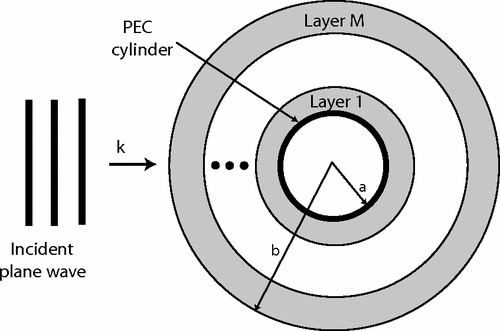
\includegraphics[height=0.25\paperheight, width=0.55\paperwidth]{fig1.png}
  \caption{Цилиндрический идеальный проводник, окруженный многослойной оболочкой
  и освещенный плоской волной. Входный и выходные радиусы оболочки есть 
  $a$ и $b$ соответственно.}
  \label{fig:1}
\end{figure}

\begin{thebibliography}{99}
\bibitem{1}J. B. Pendry, D. Schurig, and D. R. Smith, Science 312, 1780 (2006)
\end{thebibliography}

\end{document}
